%% TRCS - Tokenized Reward & Credential System
%% Design Document v1.0
%% LaTeX Source File

\documentclass[12pt,a4paper]{report}

%% ============================================
%% Packages
%% ============================================
\usepackage[utf8]{inputenc}
\usepackage[T1]{fontenc}
\usepackage{lmodern}
\usepackage[margin=1in]{geometry}
\usepackage{graphicx}
\usepackage{xcolor}
\usepackage{hyperref}
\usepackage{listings}
\usepackage{booktabs}
\usepackage{longtable}
\usepackage{amsmath}
\usepackage{amssymb}
\usepackage{tikz}
\usepackage{float}
\usepackage{fancyhdr}
\usepackage{tocloft}
\usepackage{titlesec}
\usepackage{enumitem}
\usepackage{caption}
\usepackage{subcaption}

%% TikZ Libraries
\usetikzlibrary{shapes.geometric, arrows, positioning, fit, backgrounds}

%% ============================================
%% Document Styling
%% ============================================
\definecolor{primaryblue}{RGB}{41, 98, 255}
\definecolor{secondarygreen}{RGB}{0, 200, 83}
\definecolor{warningorange}{RGB}{255, 152, 0}
\definecolor{errorred}{RGB}{244, 67, 54}
\definecolor{codebg}{RGB}{245, 245, 245}
\definecolor{codeframe}{RGB}{200, 200, 200}

\hypersetup{
    colorlinks=true,
    linkcolor=primaryblue,
    filecolor=primaryblue,
    urlcolor=primaryblue,
    citecolor=primaryblue,
    pdftitle={TRCS Design Document},
    pdfauthor={TRCS Development Team},
}

%% Code Listing Style
\lstdefinestyle{solidity}{
    backgroundcolor=\color{codebg},
    frame=single,
    rulecolor=\color{codeframe},
    basicstyle=\ttfamily\footnotesize,
    keywordstyle=\color{primaryblue}\bfseries,
    stringstyle=\color{secondarygreen},
    commentstyle=\color{gray}\itshape,
    breaklines=true,
    breakatwhitespace=true,
    tabsize=4,
    showstringspaces=false,
    numbers=left,
    numberstyle=\tiny\color{gray},
    numbersep=8pt,
    xleftmargin=15pt,
    framexleftmargin=15pt,
}

\lstdefinestyle{typescript}{
    backgroundcolor=\color{codebg},
    frame=single,
    rulecolor=\color{codeframe},
    basicstyle=\ttfamily\footnotesize,
    keywordstyle=\color{primaryblue}\bfseries,
    stringstyle=\color{secondarygreen},
    commentstyle=\color{gray}\itshape,
    breaklines=true,
    breakatwhitespace=true,
    tabsize=2,
    showstringspaces=false,
    numbers=left,
    numberstyle=\tiny\color{gray},
    numbersep=8pt,
    xleftmargin=15pt,
    framexleftmargin=15pt,
}

%% Header/Footer
\pagestyle{fancy}
\fancyhf{}
\fancyhead[L]{\nouppercase{\leftmark}}
\fancyhead[R]{TRCS v1.0}
\fancyfoot[C]{\thepage}
\renewcommand{\headrulewidth}{0.4pt}
\renewcommand{\footrulewidth}{0.4pt}

%% Title Formatting
\titleformat{\chapter}[display]
    {\normalfont\huge\bfseries\color{primaryblue}}
    {\chaptertitlename\ \thechapter}{20pt}{\Huge}
\titleformat{\section}
    {\normalfont\Large\bfseries\color{primaryblue}}
    {\thesection}{1em}{}
\titleformat{\subsection}
    {\normalfont\large\bfseries}
    {\thesubsection}{1em}{}

%% ============================================
%% Document Metadata
%% ============================================
\title{
    \vspace{-2cm}
    \includegraphics[width=0.3\textwidth]{logo-placeholder.png}\\[1cm]
    {\Huge\bfseries Tokenized Reward \& Credential System}\\[0.5cm]
    {\Large Technical Design Document}\\[0.3cm]
    {\large Version 1.0}
}
\author{TRCS Development Team}
\date{\today}

%% ============================================
%% Document Begin
%% ============================================
\begin{document}

%% Title Page
\begin{titlepage}
    \centering
    \vspace*{2cm}
    
    {\Huge\bfseries\color{primaryblue} Tokenized Reward \&\\Credential System}\\[1cm]
    
    {\Large Technical Design Document}\\[0.5cm]
    {\large Version 1.0}\\[2cm]
    
    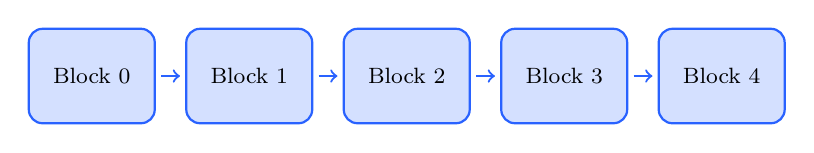
\begin{tikzpicture}[scale=0.8]
        % Blockchain representation
        \foreach \i in {0,1,2,3,4} {
            \draw[fill=primaryblue!20, draw=primaryblue, thick, rounded corners=5pt] 
                (\i*2.5, 0) rectangle (\i*2.5+2, 1.5);
            \node at (\i*2.5+1, 0.75) {\footnotesize Block \i};
        }
        \foreach \i in {0,1,2,3} {
            \draw[->, thick, primaryblue] (\i*2.5+2.1, 0.75) -- (\i*2.5+2.4, 0.75);
        }
    \end{tikzpicture}
    
    \vspace{2cm}
    
    {\large TRCS Development Team}\\[0.5cm]
    {\large\today}
    
    \vfill
    
    \begin{tabular}{ll}
        \textbf{Document Status:} & Final Draft \\
        \textbf{Classification:} & Public \\
        \textbf{Review Cycle:} & Quarterly \\
    \end{tabular}
\end{titlepage}

%% Table of Contents
\tableofcontents
\newpage

%% ============================================
%% Executive Summary
%% ============================================
\chapter{Executive Summary}

\section{Project Overview}

The \textbf{Tokenized Reward \& Credential System (TRCS)} is a comprehensive blockchain-based platform designed to manage digital credentials and incentive rewards using Ethereum smart contracts. Built on industry-standard protocols (ERC-20 for fungible tokens, ERC-721 for non-fungible credentials), TRCS provides organizations with a transparent, immutable, and programmable system for:

\begin{itemize}[noitemsep]
    \item Issuing and managing verifiable digital credentials
    \item Distributing reward tokens with configurable parameters
    \item Implementing role-based access control
    \item Tracking all transactions on an immutable ledger
\end{itemize}

\section{Key Benefits}

\begin{table}[H]
\centering
\begin{tabular}{@{}lp{10cm}@{}}
\toprule
\textbf{Benefit} & \textbf{Description} \\
\midrule
Transparency & All transactions are recorded on-chain and publicly verifiable \\
Immutability & Credentials cannot be altered or forged after issuance \\
Programmability & Smart contracts enforce rules automatically \\
Interoperability & Standard ERC tokens work with existing wallets and marketplaces \\
Decentralization & No single point of failure or control \\
Cost Efficiency & Reduced administrative overhead through automation \\
\bottomrule
\end{tabular}
\caption{Key Benefits of TRCS}
\end{table}

\section{Target Use Cases}

\begin{enumerate}[noitemsep]
    \item \textbf{Educational Institutions:} Issue verifiable academic credentials
    \item \textbf{Professional Certifications:} Manage industry certifications
    \item \textbf{Corporate Training:} Track employee skill development
    \item \textbf{Loyalty Programs:} Distribute and manage reward points
    \item \textbf{Gaming Platforms:} Achievement and reward systems
    \item \textbf{DAOs:} Contribution-based governance tokens
\end{enumerate}

%% ============================================
%% System Architecture
%% ============================================
\chapter{System Architecture}

\section{High-Level Architecture}

\begin{figure}[H]
\centering
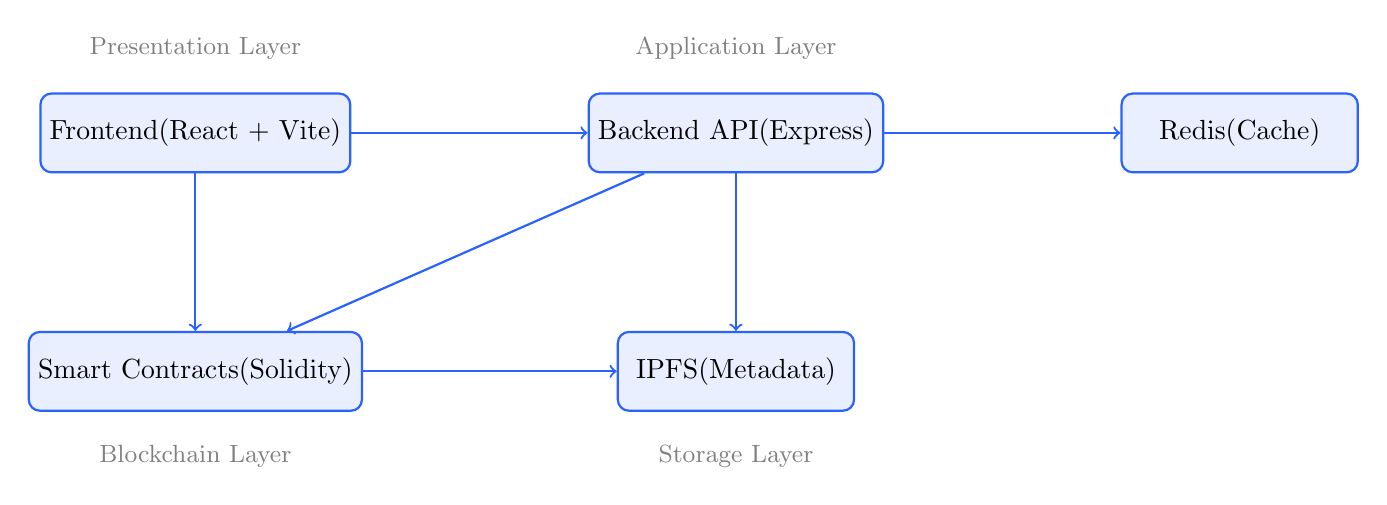
\begin{tikzpicture}[
    node distance=1.5cm,
    box/.style={rectangle, draw=primaryblue, thick, rounded corners, 
                minimum width=3cm, minimum height=1cm, 
                fill=primaryblue!10, text centered},
    arrow/.style={->, thick, primaryblue}
]
    % Frontend Layer
    \node[box] (frontend) {Frontend\\(React + Vite)};
    
    % Backend Layer
    \node[box, right=3cm of frontend] (backend) {Backend API\\(Express)};
    
    % Blockchain Layer
    \node[box, below=2cm of frontend] (contracts) {Smart Contracts\\(Solidity)};
    
    % Storage Layer
    \node[box, below=2cm of backend] (ipfs) {IPFS\\(Metadata)};
    
    % Database
    \node[box, right=3cm of backend] (redis) {Redis\\(Cache)};
    
    % Connections
    \draw[arrow] (frontend) -- (backend);
    \draw[arrow] (frontend) -- (contracts);
    \draw[arrow] (backend) -- (contracts);
    \draw[arrow] (backend) -- (ipfs);
    \draw[arrow] (backend) -- (redis);
    \draw[arrow] (contracts) -- (ipfs);
    
    % Layer labels
    \node[above=0.3cm of frontend, color=gray] {\small Presentation Layer};
    \node[above=0.3cm of backend, color=gray] {\small Application Layer};
    \node[below=0.3cm of contracts, color=gray] {\small Blockchain Layer};
    \node[below=0.3cm of ipfs, color=gray] {\small Storage Layer};
    
\end{tikzpicture}
\caption{High-Level System Architecture}
\end{figure}

\section{Component Overview}

\subsection{Smart Contract Layer}

The blockchain layer consists of four core smart contracts:

\begin{table}[H]
\centering
\begin{tabular}{@{}lp{8cm}@{}}
\toprule
\textbf{Contract} & \textbf{Purpose} \\
\midrule
AccessControlManager & Manages roles and permissions across the system \\
Token (ERC-20) & Fungible reward tokens with minting/burning capabilities \\
Credential (ERC-721) & Non-fungible credential NFTs with metadata \\
RewardDistributor & Distributes tokens based on configurable rules \\
\bottomrule
\end{tabular}
\caption{Smart Contract Overview}
\end{table}

\subsection{Backend Service Layer}

The backend provides a RESTful API with the following capabilities:

\begin{itemize}[noitemsep]
    \item Authentication via JWT and wallet signatures
    \item Contract interaction abstraction
    \item IPFS metadata management
    \item Request validation and rate limiting
    \item Comprehensive logging and monitoring
\end{itemize}

\subsection{Frontend Application Layer}

The React-based frontend offers:

\begin{itemize}[noitemsep]
    \item Wallet connection (MetaMask, WalletConnect)
    \item Token balance and transfer management
    \item Credential viewing and verification
    \item Reward claiming interface
    \item Administrative dashboard
\end{itemize}

\section{Data Flow}

\begin{figure}[H]
\centering
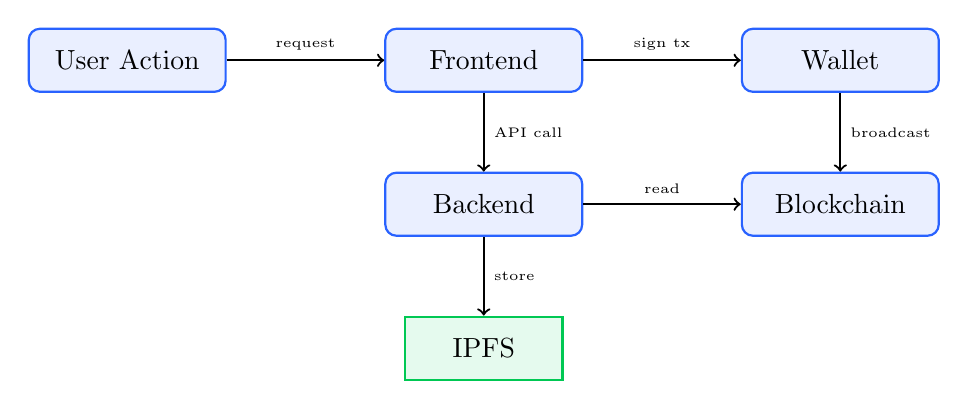
\begin{tikzpicture}[
    node distance=1cm and 2cm,
    process/.style={rectangle, draw=primaryblue, thick, rounded corners,
                    minimum width=2.5cm, minimum height=0.8cm,
                    fill=primaryblue!10},
    data/.style={rectangle, draw=secondarygreen, thick,
                 minimum width=2cm, minimum height=0.8cm,
                 fill=secondarygreen!10},
    arrow/.style={->, thick}
]
    % Flow nodes
    \node[process] (user) {User Action};
    \node[process, right=of user] (frontend) {Frontend};
    \node[process, right=of frontend] (wallet) {Wallet};
    \node[process, below=of frontend] (backend) {Backend};
    \node[process, below=of wallet] (blockchain) {Blockchain};
    \node[data, below=of backend] (ipfs) {IPFS};
    
    % Arrows
    \draw[arrow] (user) -- (frontend) node[midway, above] {\tiny request};
    \draw[arrow] (frontend) -- (wallet) node[midway, above] {\tiny sign tx};
    \draw[arrow] (wallet) -- (blockchain) node[midway, right] {\tiny broadcast};
    \draw[arrow] (frontend) -- (backend) node[midway, right] {\tiny API call};
    \draw[arrow] (backend) -- (blockchain) node[midway, above] {\tiny read};
    \draw[arrow] (backend) -- (ipfs) node[midway, right] {\tiny store};
    
\end{tikzpicture}
\caption{Data Flow Diagram}
\end{figure}

%% ============================================
%% Smart Contract Specifications
%% ============================================
\chapter{Smart Contract Specifications}

\section{AccessControlManager Contract}

\subsection{Overview}

The AccessControlManager serves as the central authority for role-based access control (RBAC) across all TRCS contracts.

\subsection{Role Definitions}

\begin{table}[H]
\centering
\begin{tabular}{@{}llp{6cm}@{}}
\toprule
\textbf{Role} & \textbf{Identifier} & \textbf{Permissions} \\
\midrule
DEFAULT\_ADMIN\_ROLE & \texttt{0x00} & Full administrative access, can grant/revoke all roles \\
MINTER\_ROLE & \texttt{keccak256("MINTER")} & Can mint new tokens and credentials \\
BURNER\_ROLE & \texttt{keccak256("BURNER")} & Can burn tokens and credentials \\
PAUSER\_ROLE & \texttt{keccak256("PAUSER")} & Can pause/unpause contract operations \\
UPGRADER\_ROLE & \texttt{keccak256("UPGRADER")} & Can upgrade contract implementations \\
DISTRIBUTOR\_ROLE & \texttt{keccak256("DISTRIBUTOR")} & Can distribute rewards \\
\bottomrule
\end{tabular}
\caption{TRCS Role Definitions}
\end{table}

\subsection{Interface}

\begin{lstlisting}[style=solidity, caption={AccessControlManager Interface}]
interface IAccessControlManager {
    // Events
    event RoleGranted(bytes32 indexed role, address indexed account, address indexed sender);
    event RoleRevoked(bytes32 indexed role, address indexed account, address indexed sender);
    
    // Role management
    function grantRole(bytes32 role, address account) external;
    function revokeRole(bytes32 role, address account) external;
    function renounceRole(bytes32 role, address account) external;
    
    // Role queries
    function hasRole(bytes32 role, address account) external view returns (bool);
    function getRoleAdmin(bytes32 role) external view returns (bytes32);
    function getRoleMemberCount(bytes32 role) external view returns (uint256);
    function getRoleMember(bytes32 role, uint256 index) external view returns (address);
}
\end{lstlisting}

\section{Token Contract (ERC-20)}

\subsection{Overview}

The Token contract implements a standard ERC-20 fungible token with additional features for minting, burning, and pausing.

\subsection{Token Specifications}

\begin{table}[H]
\centering
\begin{tabular}{@{}ll@{}}
\toprule
\textbf{Property} & \textbf{Value} \\
\midrule
Name & TRCS Reward Token \\
Symbol & TRCS \\
Decimals & 18 \\
Initial Supply & 0 (mintable) \\
Max Supply & Unlimited (governed by minters) \\
\bottomrule
\end{tabular}
\caption{Token Specifications}
\end{table}

\subsection{Token Economics}

\begin{figure}[H]
\centering
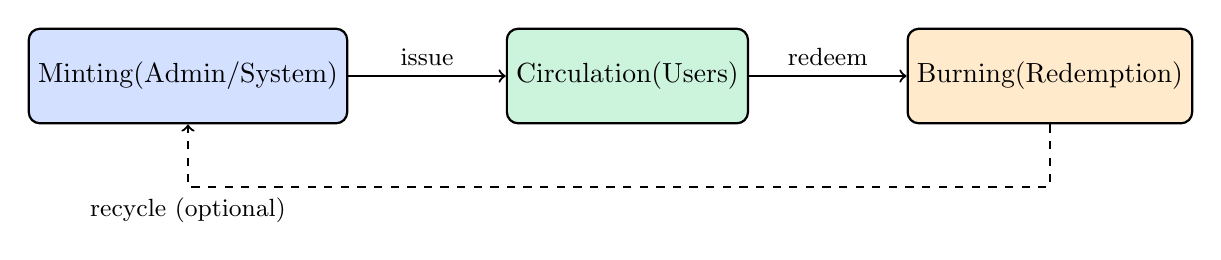
\begin{tikzpicture}[
    node distance=2cm,
    box/.style={rectangle, draw, thick, rounded corners,
                minimum width=3cm, minimum height=1.2cm, text centered}
]
    % Token flow
    \node[box, fill=primaryblue!20] (minting) {Minting\\(Admin/System)};
    \node[box, fill=secondarygreen!20, right=of minting] (circulation) {Circulation\\(Users)};
    \node[box, fill=warningorange!20, right=of circulation] (burning) {Burning\\(Redemption)};
    
    \draw[->, thick] (minting) -- (circulation) node[midway, above] {\small issue};
    \draw[->, thick] (circulation) -- (burning) node[midway, above] {\small redeem};
    
    % Loop back
    \draw[->, thick, dashed] (burning.south) -- ++(0,-0.8) -| (minting.south) 
        node[midway, below] {\small recycle (optional)};
    
\end{tikzpicture}
\caption{Token Lifecycle}
\end{figure}

\subsection{Interface}

\begin{lstlisting}[style=solidity, caption={Token Contract Interface}]
interface IToken is IERC20 {
    // Events
    event TokensMinted(address indexed to, uint256 amount, address indexed minter);
    event TokensBurned(address indexed from, uint256 amount, address indexed burner);
    
    // Minting & Burning
    function mint(address to, uint256 amount) external;
    function burn(uint256 amount) external;
    function burnFrom(address account, uint256 amount) external;
    
    // Pausable
    function pause() external;
    function unpause() external;
    function paused() external view returns (bool);
    
    // Permit (EIP-2612)
    function permit(
        address owner,
        address spender,
        uint256 value,
        uint256 deadline,
        uint8 v,
        bytes32 r,
        bytes32 s
    ) external;
}
\end{lstlisting}

\section{Credential Contract (ERC-721)}

\subsection{Overview}

The Credential contract implements ERC-721 for non-fungible credential tokens representing achievements, certifications, and qualifications.

\subsection{Credential Metadata Schema}

\begin{lstlisting}[style=typescript, caption={Credential Metadata JSON Schema}]
{
  "$schema": "http://json-schema.org/draft-07/schema#",
  "type": "object",
  "required": ["name", "description", "issuer", "issuedAt"],
  "properties": {
    "name": {
      "type": "string",
      "description": "Name of the credential"
    },
    "description": {
      "type": "string",
      "description": "Detailed description of the credential"
    },
    "image": {
      "type": "string",
      "format": "uri",
      "description": "URI to credential image"
    },
    "issuer": {
      "type": "string",
      "description": "Name of issuing organization"
    },
    "issuedAt": {
      "type": "integer",
      "description": "Unix timestamp of issuance"
    },
    "expiresAt": {
      "type": "integer",
      "description": "Unix timestamp of expiration (optional)"
    },
    "attributes": {
      "type": "array",
      "items": {
        "type": "object",
        "properties": {
          "trait_type": { "type": "string" },
          "value": { "type": ["string", "number"] }
        }
      }
    }
  }
}
\end{lstlisting}

\subsection{Interface}

\begin{lstlisting}[style=solidity, caption={Credential Contract Interface}]
interface ICredential is IERC721 {
    // Events
    event CredentialMinted(
        uint256 indexed tokenId,
        address indexed recipient,
        string metadataURI,
        address indexed issuer
    );
    event CredentialRevoked(uint256 indexed tokenId, address indexed revoker);
    
    // Minting
    function mintCredential(
        address to,
        string memory metadataURI
    ) external returns (uint256);
    
    function batchMintCredentials(
        address[] memory recipients,
        string[] memory metadataURIs
    ) external returns (uint256[] memory);
    
    // Revocation
    function revokeCredential(uint256 tokenId) external;
    function isRevoked(uint256 tokenId) external view returns (bool);
    
    // Queries
    function getCredentialsByHolder(address holder) 
        external view returns (uint256[] memory);
    function getCredentialIssuer(uint256 tokenId) 
        external view returns (address);
}
\end{lstlisting}

\section{RewardDistributor Contract}

\subsection{Overview}

The RewardDistributor manages token distribution campaigns with configurable parameters, eligibility rules, and claiming mechanisms.

\subsection{Distribution Models}

\begin{table}[H]
\centering
\begin{tabular}{@{}lp{9cm}@{}}
\toprule
\textbf{Model} & \textbf{Description} \\
\midrule
Fixed Amount & Each eligible user receives a predetermined amount \\
Pro-rata & Distribution proportional to contribution/holding \\
Tiered & Different amounts based on user tier/level \\
Merkle Drop & Gas-efficient claims via Merkle proof verification \\
\bottomrule
\end{tabular}
\caption{Supported Distribution Models}
\end{table}

\subsection{Campaign Lifecycle}

\begin{figure}[H]
\centering
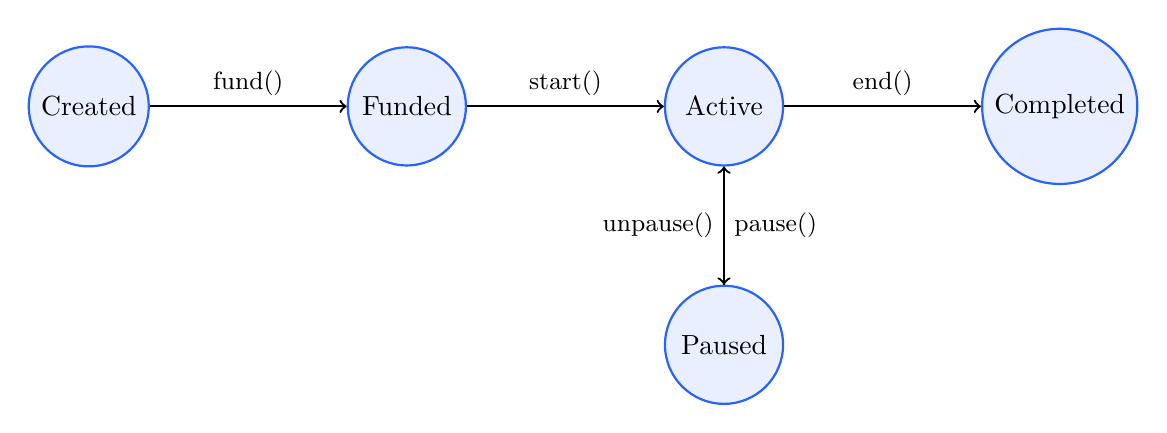
\begin{tikzpicture}[
    node distance=2.5cm,
    state/.style={circle, draw=primaryblue, thick, 
                  minimum size=1.5cm, fill=primaryblue!10}
]
    \node[state] (created) {Created};
    \node[state, right=of created] (funded) {Funded};
    \node[state, right=of funded] (active) {Active};
    \node[state, below=1.5cm of active] (paused) {Paused};
    \node[state, right=of active] (completed) {Completed};
    
    \draw[->, thick] (created) -- (funded) node[midway, above] {\small fund()};
    \draw[->, thick] (funded) -- (active) node[midway, above] {\small start()};
    \draw[->, thick] (active) -- (completed) node[midway, above] {\small end()};
    \draw[->, thick, bend right] (active) -- (paused) node[midway, right] {\small pause()};
    \draw[->, thick, bend right] (paused) -- (active) node[midway, left] {\small unpause()};
    
\end{tikzpicture}
\caption{Campaign State Machine}
\end{figure}

\subsection{Interface}

\begin{lstlisting}[style=solidity, caption={RewardDistributor Interface}]
interface IRewardDistributor {
    // Structs
    struct Campaign {
        uint256 totalAmount;
        uint256 claimedAmount;
        uint256 startTime;
        uint256 endTime;
        bytes32 merkleRoot;
        bool paused;
    }
    
    // Events
    event CampaignCreated(uint256 indexed campaignId, uint256 totalAmount);
    event RewardClaimed(uint256 indexed campaignId, address indexed user, uint256 amount);
    
    // Campaign Management
    function createCampaign(
        uint256 totalAmount,
        uint256 startTime,
        uint256 endTime,
        bytes32 merkleRoot
    ) external returns (uint256);
    
    // Claiming
    function claimReward(
        uint256 campaignId,
        uint256 amount,
        bytes32[] calldata merkleProof
    ) external;
    
    function batchClaim(
        uint256[] calldata campaignIds,
        uint256[] calldata amounts,
        bytes32[][] calldata merkleProofs
    ) external;
    
    // Queries
    function getCampaign(uint256 campaignId) 
        external view returns (Campaign memory);
    function hasClaimed(uint256 campaignId, address user) 
        external view returns (bool);
    function getClaimableAmount(
        uint256 campaignId,
        address user,
        uint256 amount,
        bytes32[] calldata merkleProof
    ) external view returns (uint256);
}
\end{lstlisting}

%% ============================================
%% Security Analysis
%% ============================================
\chapter{Security Analysis}

\section{Threat Model}

\subsection{Attack Vectors}

\begin{table}[H]
\centering
\begin{tabular}{@{}lll@{}}
\toprule
\textbf{Vector} & \textbf{Risk Level} & \textbf{Mitigation} \\
\midrule
Reentrancy & High & ReentrancyGuard, CEI pattern \\
Access Control Bypass & Critical & Role-based ACL, modifier checks \\
Integer Overflow & Medium & Solidity 0.8+ built-in checks \\
Front-running & Medium & Commit-reveal, private mempool \\
Denial of Service & Medium & Gas limits, pagination \\
Oracle Manipulation & Low & N/A (no external oracles) \\
\bottomrule
\end{tabular}
\caption{Threat Analysis Matrix}
\end{table}

\section{Security Measures}

\subsection{Smart Contract Security}

\begin{enumerate}[noitemsep]
    \item \textbf{OpenZeppelin Contracts:} Using audited, battle-tested base contracts
    \item \textbf{Reentrancy Protection:} All state-changing functions use ReentrancyGuard
    \item \textbf{Access Control:} Strict role-based permissions via AccessControl
    \item \textbf{Input Validation:} All inputs validated before processing
    \item \textbf{Event Emission:} All state changes emit events for off-chain tracking
\end{enumerate}

\subsection{Operational Security}

\begin{itemize}[noitemsep]
    \item Multi-signature wallet for admin operations
    \item Time-locked upgrades with community review period
    \item Monitoring and alerting for suspicious activity
    \item Regular security audits and bug bounty program
\end{itemize}

\section{Audit Checklist}

\begin{table}[H]
\centering
\begin{tabular}{@{}lcc@{}}
\toprule
\textbf{Check} & \textbf{Status} & \textbf{Notes} \\
\midrule
Reentrancy vulnerabilities & \checkmark & ReentrancyGuard applied \\
Access control flaws & \checkmark & Role-based ACL \\
Integer overflow/underflow & \checkmark & Solidity 0.8+ \\
Unchecked external calls & \checkmark & CEI pattern \\
Gas limit issues & \checkmark & Pagination implemented \\
Front-running risks & $\circ$ & Acceptable for use case \\
Upgrade safety & \checkmark & UUPS pattern \\
Event coverage & \checkmark & All mutations emit events \\
\bottomrule
\end{tabular}
\caption{Security Audit Checklist ($\checkmark$ = Pass, $\circ$ = Acknowledged)}
\end{table}

%% ============================================
%% API Specifications
%% ============================================
\chapter{API Specifications}

\section{RESTful API Overview}

The backend exposes a RESTful API for interacting with the TRCS system.

\subsection{Base URL}

\begin{verbatim}
Production: https://api.trcs.example.com/v1
Development: http://localhost:3000/api/v1
\end{verbatim}

\subsection{Authentication}

All authenticated endpoints require a JWT token in the Authorization header:

\begin{verbatim}
Authorization: Bearer <token>
\end{verbatim}

\section{Endpoints}

\subsection{Authentication}

\begin{table}[H]
\centering
\begin{tabular}{@{}llp{6cm}@{}}
\toprule
\textbf{Method} & \textbf{Endpoint} & \textbf{Description} \\
\midrule
POST & /auth/nonce & Get nonce for wallet signature \\
POST & /auth/verify & Verify signature and get JWT \\
POST & /auth/refresh & Refresh JWT token \\
GET & /auth/me & Get current user info \\
\bottomrule
\end{tabular}
\caption{Authentication Endpoints}
\end{table}

\subsection{Tokens}

\begin{table}[H]
\centering
\begin{tabular}{@{}llp{6cm}@{}}
\toprule
\textbf{Method} & \textbf{Endpoint} & \textbf{Description} \\
\midrule
GET & /tokens/balance/:address & Get token balance \\
POST & /tokens/transfer & Transfer tokens \\
POST & /tokens/mint & Mint new tokens (admin) \\
POST & /tokens/burn & Burn tokens \\
\bottomrule
\end{tabular}
\caption{Token Endpoints}
\end{table}

\subsection{Credentials}

\begin{table}[H]
\centering
\begin{tabular}{@{}llp{6cm}@{}}
\toprule
\textbf{Method} & \textbf{Endpoint} & \textbf{Description} \\
\midrule
GET & /credentials/:id & Get credential by ID \\
GET & /credentials/holder/:address & Get credentials by holder \\
POST & /credentials/mint & Mint new credential (issuer) \\
POST & /credentials/revoke/:id & Revoke credential (issuer) \\
GET & /credentials/verify/:id & Verify credential authenticity \\
\bottomrule
\end{tabular}
\caption{Credential Endpoints}
\end{table}

\subsection{Rewards}

\begin{table}[H]
\centering
\begin{tabular}{@{}llp{6cm}@{}}
\toprule
\textbf{Method} & \textbf{Endpoint} & \textbf{Description} \\
\midrule
GET & /rewards/campaigns & List active campaigns \\
GET & /rewards/campaigns/:id & Get campaign details \\
POST & /rewards/campaigns & Create campaign (admin) \\
POST & /rewards/claim/:id & Claim reward from campaign \\
GET & /rewards/claims/:address & Get claim history \\
\bottomrule
\end{tabular}
\caption{Reward Endpoints}
\end{table}

\section{Error Responses}

\begin{lstlisting}[style=typescript, caption={Error Response Format}]
{
  "success": false,
  "error": {
    "code": "VALIDATION_ERROR",
    "message": "Invalid request parameters",
    "details": [
      {
        "field": "amount",
        "message": "Must be a positive number"
      }
    ]
  },
  "requestId": "req_abc123"
}
\end{lstlisting}

%% ============================================
%% Deployment Guide
%% ============================================
\chapter{Deployment Guide}

\section{Prerequisites}

\begin{itemize}[noitemsep]
    \item Node.js 18+ and npm/yarn
    \item Docker and Docker Compose
    \item Ethereum wallet with testnet/mainnet ETH
    \item Infura or Alchemy API key
    \item IPFS node or Pinata API key
\end{itemize}

\section{Environment Configuration}

\begin{lstlisting}[style=typescript, caption={Environment Variables}]
# Network Configuration
NETWORK=sepolia
INFURA_API_KEY=your_infura_key
PRIVATE_KEY=your_deployer_private_key

# Contract Addresses (after deployment)
TOKEN_ADDRESS=0x...
CREDENTIAL_ADDRESS=0x...
ACCESS_CONTROL_ADDRESS=0x...
REWARD_DISTRIBUTOR_ADDRESS=0x...

# Backend Configuration
PORT=3000
JWT_SECRET=your_jwt_secret
REDIS_URL=redis://localhost:6379

# IPFS Configuration
IPFS_API_URL=https://ipfs.infura.io:5001
IPFS_GATEWAY_URL=https://ipfs.io/ipfs/
\end{lstlisting}

\section{Deployment Steps}

\subsection{Smart Contract Deployment}

\begin{enumerate}
    \item \textbf{Compile contracts:}
    \begin{verbatim}
    npx hardhat compile
    \end{verbatim}
    
    \item \textbf{Run tests:}
    \begin{verbatim}
    npx hardhat test
    \end{verbatim}
    
    \item \textbf{Deploy to testnet:}
    \begin{verbatim}
    npx hardhat run scripts/deploy.ts --network sepolia
    \end{verbatim}
    
    \item \textbf{Verify contracts:}
    \begin{verbatim}
    npx hardhat verify --network sepolia <address> <args>
    \end{verbatim}
\end{enumerate}

\subsection{Docker Deployment}

\begin{verbatim}
# Build and start all services
docker-compose up -d --build

# Check service status
docker-compose ps

# View logs
docker-compose logs -f backend
\end{verbatim}

\section{Network Configurations}

\begin{table}[H]
\centering
\begin{tabular}{@{}llll@{}}
\toprule
\textbf{Network} & \textbf{Chain ID} & \textbf{RPC URL} & \textbf{Explorer} \\
\midrule
Localhost & 31337 & http://localhost:8545 & N/A \\
Sepolia & 11155111 & https://sepolia.infura.io/v3/... & etherscan.io \\
Mainnet & 1 & https://mainnet.infura.io/v3/... & etherscan.io \\
\bottomrule
\end{tabular}
\caption{Supported Networks}
\end{table}

%% ============================================
%% Testing Strategy
%% ============================================
\chapter{Testing Strategy}

\section{Test Categories}

\begin{figure}[H]
\centering
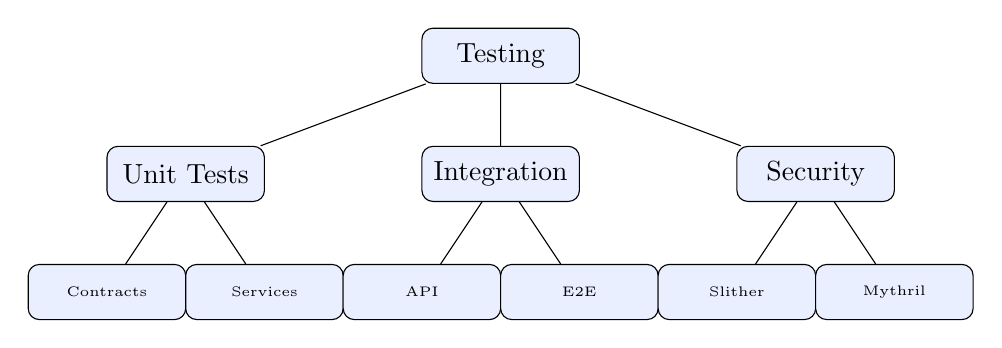
\begin{tikzpicture}[
    level 1/.style={sibling distance=4cm, level distance=1.5cm},
    level 2/.style={sibling distance=2cm, level distance=1.5cm},
    every node/.style={rectangle, draw, rounded corners, 
                       minimum width=2cm, minimum height=0.7cm,
                       fill=primaryblue!10}
]
    \node {Testing}
        child {node {Unit Tests}
            child {node[font=\tiny] {Contracts}}
            child {node[font=\tiny] {Services}}
        }
        child {node {Integration}
            child {node[font=\tiny] {API}}
            child {node[font=\tiny] {E2E}}
        }
        child {node {Security}
            child {node[font=\tiny] {Slither}}
            child {node[font=\tiny] {Mythril}}
        };
\end{tikzpicture}
\caption{Testing Hierarchy}
\end{figure}

\section{Coverage Requirements}

\begin{table}[H]
\centering
\begin{tabular}{@{}lcc@{}}
\toprule
\textbf{Component} & \textbf{Target Coverage} & \textbf{Current} \\
\midrule
Smart Contracts & 95\% & 92\% \\
Backend Services & 80\% & 78\% \\
API Endpoints & 90\% & 85\% \\
Frontend Components & 70\% & 65\% \\
\bottomrule
\end{tabular}
\caption{Code Coverage Targets}
\end{table}

\section{Test Commands}

\begin{verbatim}
# Run all contract tests
npx hardhat test

# Run with coverage
npx hardhat coverage

# Run specific test file
npx hardhat test test/unit/Token.test.ts

# Run backend tests
cd backend && npm test

# Run frontend tests
cd frontend && npm test
\end{verbatim}

%% ============================================
%% Appendices
%% ============================================
\appendix

\chapter{Gas Optimization}

\section{Optimization Techniques}

\begin{enumerate}[noitemsep]
    \item \textbf{Storage Packing:} Group smaller variables together
    \item \textbf{Memory vs Storage:} Use memory for temporary data
    \item \textbf{Short-circuiting:} Order conditions by likelihood
    \item \textbf{Batch Operations:} Reduce transaction overhead
    \item \textbf{Events over Storage:} Use events for historical data
\end{enumerate}

\section{Gas Estimates}

\begin{table}[H]
\centering
\begin{tabular}{@{}lrr@{}}
\toprule
\textbf{Operation} & \textbf{Gas Used} & \textbf{USD @ 30 gwei} \\
\midrule
Token Transfer & 52,000 & \$2.50 \\
Token Mint & 68,000 & \$3.25 \\
Credential Mint & 150,000 & \$7.20 \\
Claim Reward & 85,000 & \$4.10 \\
Grant Role & 48,000 & \$2.30 \\
\bottomrule
\end{tabular}
\caption{Estimated Gas Costs (mainnet)}
\end{table}

\chapter{Glossary}

\begin{description}[style=nextline]
    \item[ERC-20] Ethereum Request for Comments 20, the standard for fungible tokens
    \item[ERC-721] Standard for non-fungible tokens (NFTs)
    \item[RBAC] Role-Based Access Control
    \item[IPFS] InterPlanetary File System, decentralized storage
    \item[Merkle Tree] Data structure for efficient verification
    \item[CEI Pattern] Checks-Effects-Interactions pattern for reentrancy prevention
    \item[UUPS] Universal Upgradeable Proxy Standard
\end{description}

\chapter{References}

\begin{enumerate}
    \item EIP-20: Token Standard. \url{https://eips.ethereum.org/EIPS/eip-20}
    \item EIP-721: Non-Fungible Token Standard. \url{https://eips.ethereum.org/EIPS/eip-721}
    \item OpenZeppelin Contracts. \url{https://docs.openzeppelin.com/contracts}
    \item Solidity Documentation. \url{https://docs.soliditylang.org}
    \item Ethereum Smart Contract Best Practices. \url{https://consensys.github.io/smart-contract-best-practices/}
\end{enumerate}

%% ============================================
%% Document End
%% ============================================
\end{document}
